\section{Response due to moving loads}
\label{sec:moving_loads_response}

Finally, we can simulate a real working condition for the harbour crane, by applying a moving load on the structure.

In particular, we can consider a mass of $m = 45[T]$ moving along the $x$ axis, starting from the correspondence of node \textbf{\#7} and moving towards node \textbf{\#9} (tip of the arm crane).

\subsection{Trapezoidal motion profile}
\label{subsec:trapezoidal_motion_profile}

As for the motion type of the mass along the $x$ axis, we can consider a trapezoidal velocity profile, with a constant acceleration phase, a constant velocity phase, and a constant deceleration phase.
In particular, if we consider the total distance covered by the mass as $L = 24[m]$ and a total time of $T = 20[s]$, we can compute both the accelerations ($a_{acc} = |a_{dec}| = a$), velocity ($v_{max}$), and the time duration of each phase ($t_1$, $t_2$ and $t_3$):

\begin{equation}
    \begin{cases}
        L = \frac{1}{2} \cdot a \cdot t_1^2 + v_{max} \cdot t_2 + \frac{1}{2} \cdot |a| \cdot t_3^2 \\
        T = t_1 + t_2 + t_3
    \end{cases}
\end{equation}

By solving the system of equations, we can find the following values:

\begin{equation}
    \begin{cases}
        a = 0.25 [m/s^2]  \\
        v_{max} = 2 [m/s] \\
        t_1 = 8 [s]       \\
        t_2 = 4 [s]       \\
        t_3 = 8 [s]
    \end{cases}
\end{equation}

Once the position of the load over time is computed, we must compute the equivalent nodal forces that is applied to the structure because of the load.

For simplicity, we neglect any nodal momentum, and we just consider the vertical nodal force.
By doing so, we can compute the equivalent nodal force by solving the following equations:

\begin{align}
    \xi           & = \frac{x - x_1}{x_2 - x_1} \\
    \mathbf{F_{F, eq, left}}  & = m \cdot g \cdot \xi       \\
    \mathbf{F_{F, eq, right}} & = m \cdot g \cdot (1 - \xi)
    \label{eq:equivalent_nodal_force}
\end{align}

Where $x$ is the position of the mass, $x_1$ and $x_2$ are the position of the two nodes that are closest to the mass, and $g$ is the gravity acceleration.

Once the nodal forces are known for each time step, we can compute the nodal displacements by solving the partial differential equation that describes the motion of the structure:

\begin{equation}
    [M_{FF}] \cdot \mathbf{\ddot{X}}(t) + [C_{FF}] \cdot \mathbf{\dot{X}}(t) + [K_{FF}] \cdot \mathbf{X}(t) = \mathbf{F_{F, eq}}(t)
    \label{eq:dynamic_equation}
\end{equation}

Where $[M_{FF}]$, $[C_{FF}]$ and $[K_{FF}]$ are the mass, damping and stiffness matrices of the structure, $\mathbf{X}$ is the nodal displacement vector, and $\mathbf{F_{F, eq}}$ is the equivalent nodal force vector.

To solve the equation, we must rely on a numerical method, such as the `Runge-Kutta' method, that allows us to solve the equation for each time step.

\subsection{Initial conditions}
\label{subsec:initial_conditions}

One important aspect about this type of analysis is the initial conditions of the structure.

In particular, we can consider two different initial conditions:

\begin{itemize}
    \item \textbf{Initial condition 1}: the structure is in its undeformed configuration, and the load is suddenly added to the structure and starts moving.
    \item \textbf{Initial condition 2}: the structure is in its deformed configuration due to the static loads of the mass, which then starts to move along the $x$ axis.
\end{itemize}

As we can imagine, the first set of initial conditions will lead to a much more complex dynamic response since it will be the superposition of the fast dynamic response due to the sudden addition of the load (oscillatory behavior) and the slow dynamic response due to the moving load.
On the other hand, the second set of initial conditions will lead to a cleaner and calm dynamic response, since the structure starts from a condition much more similar to the final condition.
\subsection{Implementation}
\label{subsec:implementation}

Before proceeding with the discussion about the results, we report here the code implementation used to perform the dynamic analysis of the structure due to the moving load.

Using \texttt{MATLAB}, the code is the following:

\begin{lstlisting}[language=Matlab, caption={Implementation of the moving load dynamic analysis.}]
    load_position = @(t) ...
        (t <= t1) .*                             (1/2 * a * t.^2) + ...
        (t > t1 & t <= (t1 + t2)) .*             (1/2 * a * t1^2 + v * (t - t1)) + ...
        (t > (t1 + t2) & t <= (t1 + t2 + t3)) .* (1/2 * a * t1^2 + v * t2 + v * (t - (t2 + t1)) - 1/2 * a * (t - (t1 + t2)).^2) + ...
        (t > (t1 + t2 + t3)) .*                  (1/2 * a * t1^2 + v * t2 + v * t3 - 1/2 * a * t3.^2);

    Q_func = @(t) Phi' * compute_nodal_load(load_position(t), xy, idb, -9.81 * 40e3);

    initial_conditions = [zeros(length(Q_func(0)), 1) zeros(length(Q_func(0)), 1)];
    initial_conditions = [zeros(length(Q_func(0)), 1) K_FF_modal \ Q_func(0)];

    [t, z] = ode45( ...
        @(t, z) EquationOfMotion(t, z, M_FF_modal, C_FF_modal, K_FF_modal, Q_func), ...
        [0 max(t_vet)], ...
        initial_conditions, ...
        odeset('RelTol', 1e-6, 'AbsTol', 1e-6));

    X_moving_load = Phi * z(:, size(Phi, 2)+1:end)';

    %% Functions

    function [z_dot] = EquationOfMotion(t, z, M_FF_modal, C_FF_modal, K_FF_modal, Q_func)

        N_considered_modes = size(K_FF_modal, 1);

        q_dot = z(1:N_considered_modes, 1);
        q = z(N_considered_modes + (1:N_considered_modes), 1);

        % M * x_dot_dot + C * x_dot + K * x = F(t) -> Modal coordinates -> q
        q_dot_dot = M_FF_modal \ (Q_func(t) - C_FF_modal * q_dot - K_FF_modal * q);

        z_dot(1:N_considered_modes, 1) = q_dot_dot;
        z_dot(N_considered_modes + (1:N_considered_modes), 1) = q_dot;

    end


    function F_nodal = compute_nodal_load(load_position, xy, idb, F0)
    % Strictly related to our case at hand, nodes D to A.

        F_nodal = zeros(71, 1);

        if (load_position + xy(7, 1) < xy(8, 1))

            L = xy(8, 1) - xy(7, 1);
            xi = (load_position) / L;

            N1 = 1 - xi;
            N2 = xi;

            F_nodal(idb(7, 2)) = F0 * N1;
            F_nodal(idb(8, 2)) = F0 * N2;

        else

            L = xy(9, 1) - xy(8, 1);
            xi = (load_position - (xy(8, 1) - xy(7, 1))) / L;

            N1 = 1 - xi;
            N2 = xi;

            F_nodal(idb(8, 2)) = F0 * N1;
            F_nodal(idb(9, 2)) = F0 * N2;

        end

end

\end{lstlisting}

\subsection{Results}
\label{subsec:results}

In this section, we will show the results of the dynamic analysis of the structure due to the moving load, considering both the cases of initial conditions as explained in the previous section.

\paragraph{Initial condition 1}

In this case, the structure is in its undeformed configuration, and the load is suddenly added to the structure and starts moving at $t = 0$.

\begin{figure}[H]
    \centering
    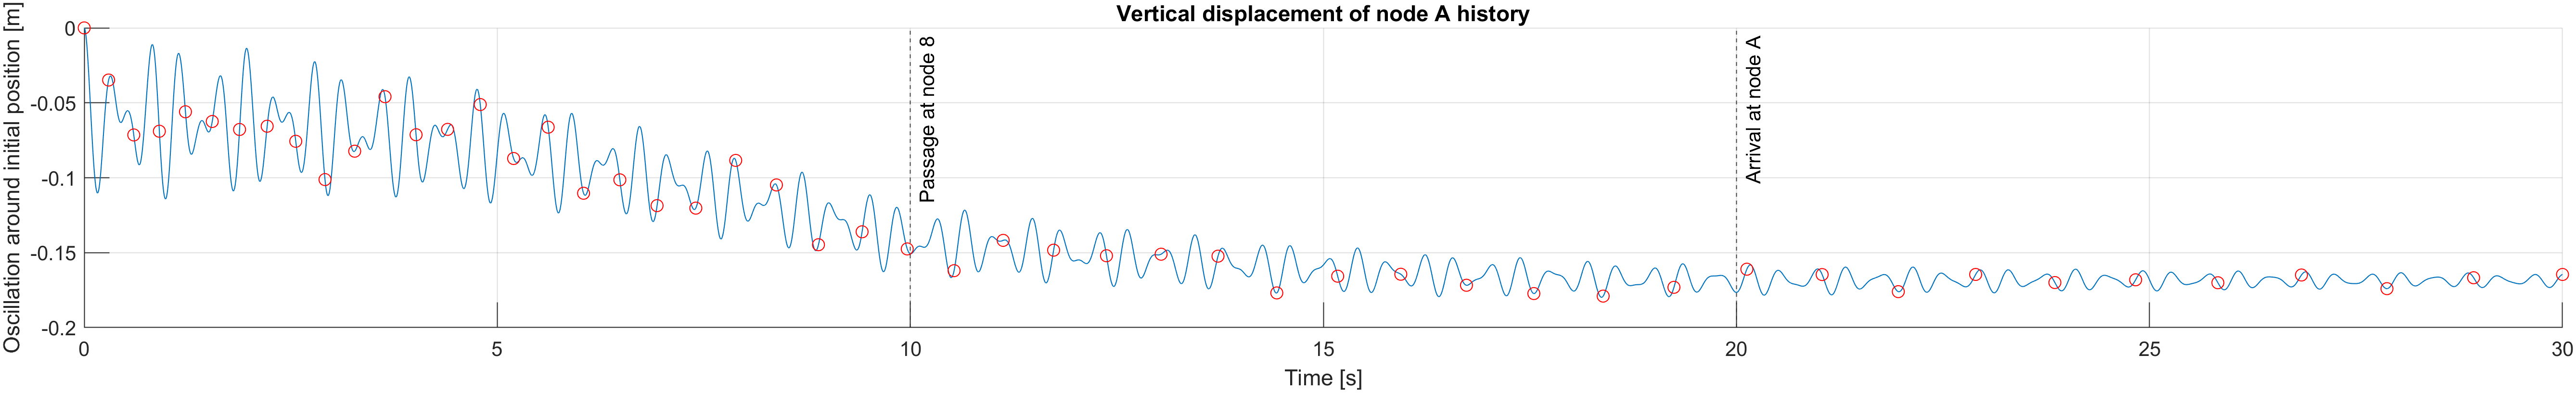
\includegraphics[width=\textwidth]{img/MATLAB/Responses/Moving_load_history_condition_1.png}
    \caption{Dynamic response of the structure due to the moving load (initial condition 1)}
    \label{fig:moving_loads_response_initial_condition_1}
\end{figure}

As we can see from the time history of node A, the structure shows a fast dynamic response due to the sudden addition of the load (in some sense this might be seen as a shock/impact response), over imposed to a slow dynamic response due to the moving load.

\paragraph{Initial condition 2}

In this case, the structure is in its deformed configuration due to the static loads of the mass, which then starts to move along the $x$ axis at $t = 0$.

\begin{figure}[H]
    \centering
    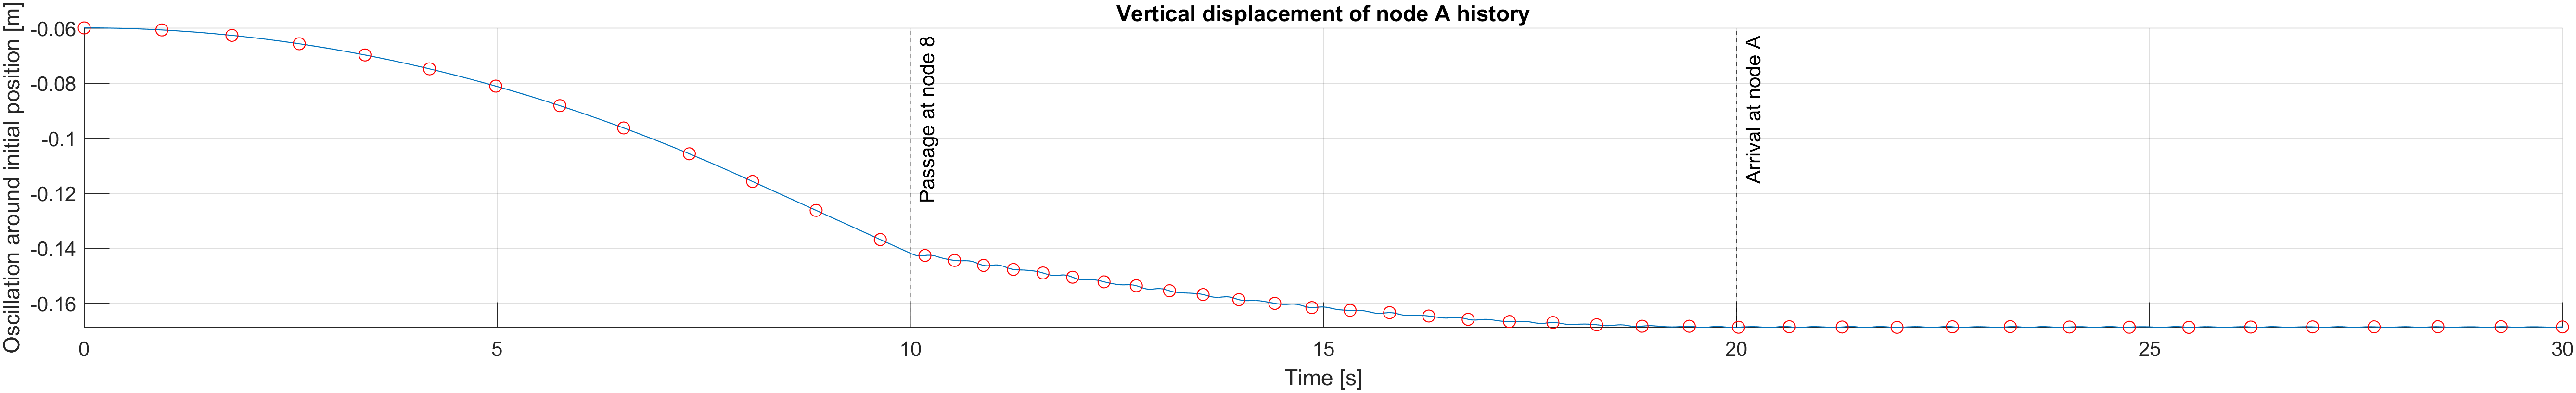
\includegraphics[width=\textwidth]{img/MATLAB/Responses/Moving_load_history_condition_2.png}
    \caption{Dynamic response of the structure due to the moving load (initial condition 2)}
    \label{fig:moving_loads_response_initial_condition_2}
\end{figure}

As we can see from the time history of node A, the structure shows a much more steady and controlled response, with no strong oscillatory behavior.
This can be explained by the absence of the equivalent shock/impact response due to the sudden addition of the load.

